\section{Preliminaries}
\label{sec:prelim}

% \subsection{Terminology}
% Here, we define the terminology used in this paper.

% 1. \textit{Configuration parameter}, or \textit{parameter} for short, is a variable that is used to configure the behavior of a software system. For example, the \texttt{client} parameter in LineairDB is used to configure the number of threads that can concurrently access the database. We use the term \textit{configuration} to denote a set of all parameters.

% 2. \textit{Environment} is a hardware setup in which a DBMS runs. 
% Source environment denotes the environment where we can readily measure the performance of a DBMS.
% Target environment is where we want to build a performance prediction model for. 
% We use the knowledge obtained from the source environment to build a model for the target environment.

% 3. \textit{Performance function} is the true relationship between the performance of a DBMS and its configuration. 
% \textit{Performance prediction model} approximates the performance function based on available data.
% $f_{env}(\boldsymbol{p_i})$ represents the performance function in an environment $env$ when a parameter is set to $\boldsymbol{p_i}$ and other parameters are set to their default values.

\subsection{Transfer Learning}
\label{sec:prelim:tl}
Transfer learning is an active research area that aims to reduce the cost of building a model by utilizing the knowledge obtained from a different but related source.
In this paper, we compare with the transfer learning techniques that have been proposed for the performance prediction of configurable software systems.

1. \textit{ModelShift} is a type of transfer learning where the performance model learned from the source environment is linearly transformed to predict the performance of the target environment\cite{Valov}. Essentially, this method constructs a linear regression model that reflects the relationship between the performance of the source and target environments, as in Fig.~\ref{fig:valov}. Previous study has shown that ModelShift requires less than 10 samples from the target environment to learn the linear regression model\cite{Valov}. 

2. \textit{DataReuseTL} is an approach to use the source environment data in addition to data samples from the target environment to build a performance prediction model\cite{datareuse}. 
DataReuseTL works especially well even with few samples from the target environment when the source and target environments have small differences.

3. \textit{L2S} extracts information that are likely to be shared between the source and target environments\cite{jamshidi}, and uses them to build a model for the target environment\cite{l2s}.
Because this method does not use the source environment data for model construction, there are no concerns about the bias caused by the difference between the source and target environments.

\subsection{Limitations of Existing Transfer Learning Methods}
\label{sec:prelim:limitation}

\begin{figure*}[htbp]
  \centering
  \begin{minipage}{.4\textwidth}
    \centering
    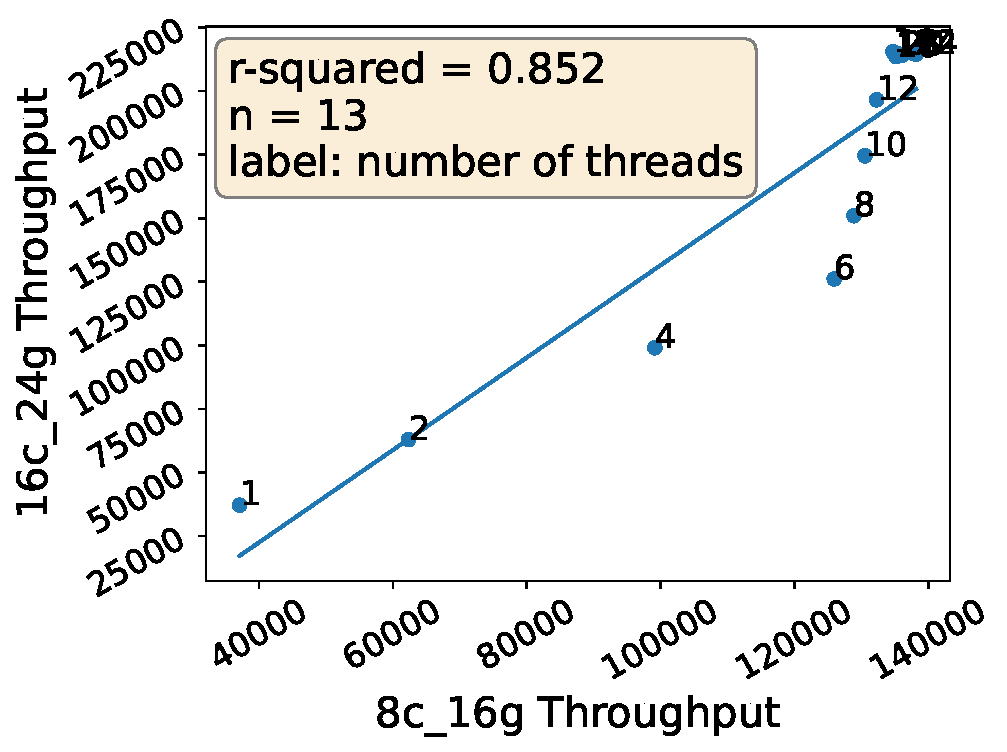
\includegraphics[width=.7\linewidth]{src/fig/rw8_vs_16.pdf}
    \caption{\textbf{Relationship of LineairDB\cite{lineairdb} throughput between two environments and a linear regression model} -- The label on each point shows the value of the parameter. The x-axis represents the throughput of 8 core 16 GB memory machine while the y-axis represents the throughput of 16 core 24 GB memory machine.}
    \label{fig:valov}
  \end{minipage}%
  \hfill
  \begin{minipage}{.55\textwidth}
    \centering
    \subfloat[Linear parameter]{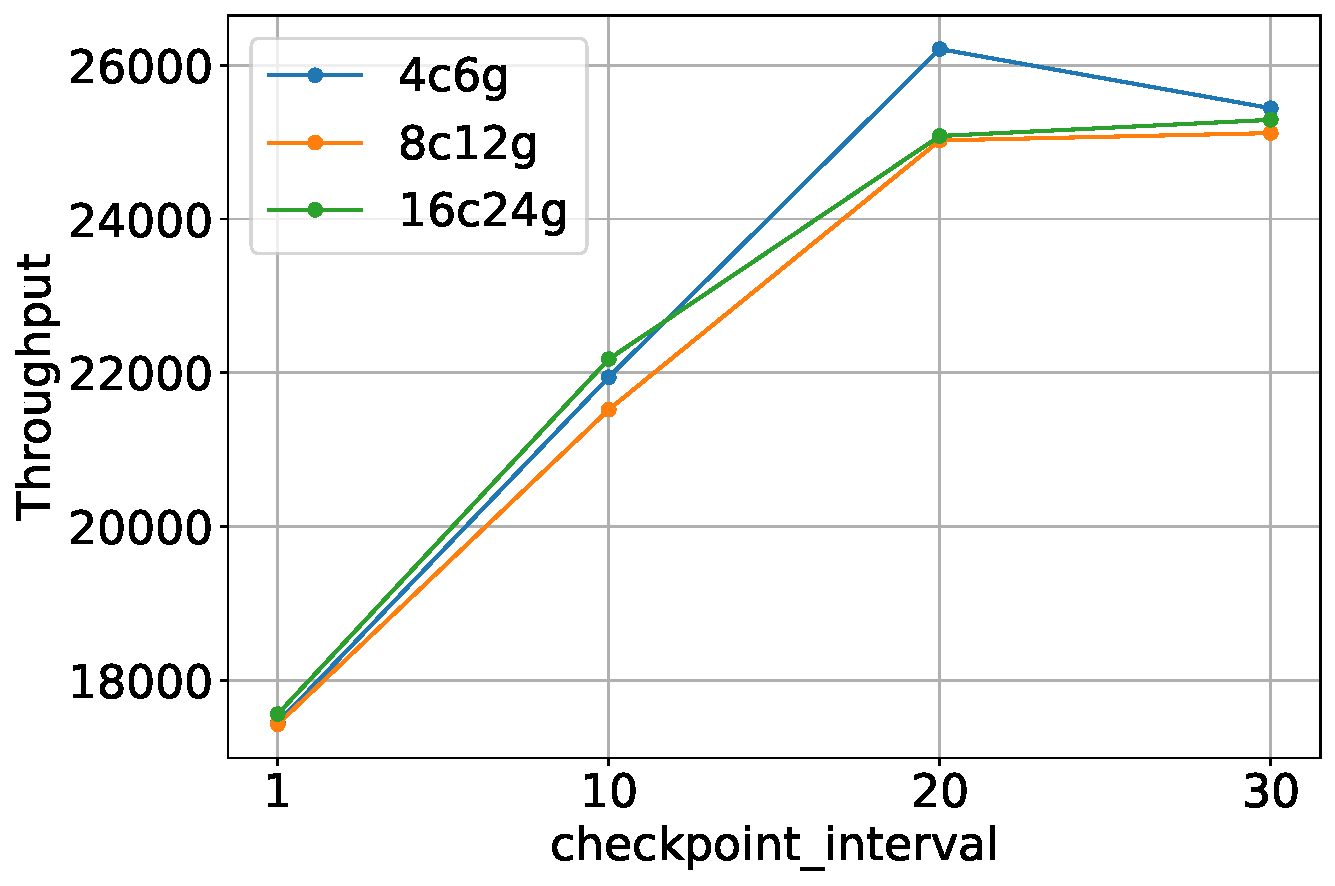
\includegraphics[width=.45\linewidth]{src/fig/checkpoint_interval.pdf}\label{fig:param:related}}
    \hfill
    \subfloat[Non-linear parameter]{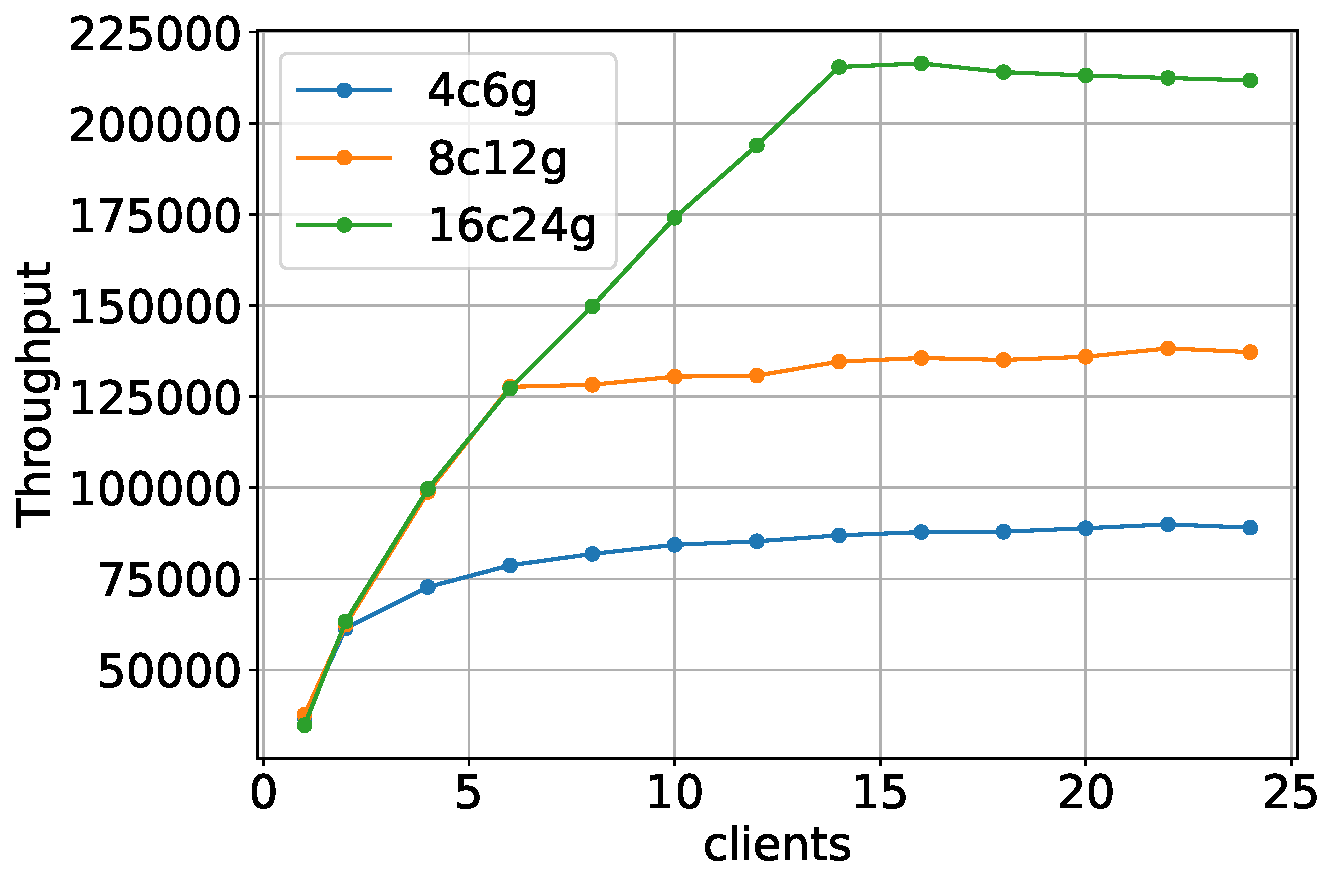
\includegraphics[width=.45\linewidth]{src/fig/clients.pdf}\label{fig:param:independent}}
    \caption{\textbf{Performance functions of linear and non-linear parameters} -- Each line represents the performance function of a parameter in a different environment. For example, 4c6g represents the performance function of a parameter in an environment with 4 CPU cores and 6 GB of memory.}
    \label{fig:params}
  \end{minipage}
\end{figure*}

Parameters in DBMS (and other configurable software systems) can be categorized into two types: \textit{linear} and \textit{non-linear}.

Linear parameters are the parameters that affect the performance of a DBMS similarly in different environments.
Formally, a parameter $\boldsymbol{p_i}$ is linear if it satisfies the following equation:
\begin{equation}
    f_{tgt}(\boldsymbol{p_i}) = \beta{\times}f_{src}(\boldsymbol{p_i})+\beta_0\label{linear}
\end{equation}
where $f_{tgt}(\boldsymbol{p_i})$ represents the performance function in a target environment, and $\beta{\times}f_{src}(\boldsymbol{p_i})+\beta_0$ denotes a linear transformation of the performance function in a source environment.
Fig.~\ref{fig:param:related} shows an example of a linear parameter in LineairDB.
The figure shows that the performance function of the parameter have similar shapes in different environments, and that the performance in one environment can be approximated by linearly transforming the performance in another environment.
This result suggests that source environment data of linear parameters can be readily reused after an appropriate linear transformation to build a model for the target environment.
Considering that it takes less than 10 samples from the target environment to learn the linear transformation\cite{Valov}, the data of linear parameters from the source environment should be exploited in order to build a model using fewer samples from the target environment.

The remaining parameters are non-linear parameters that behave differently in different environments.
Fig.~\ref{fig:param:independent} shows an example of a non-linear parameter.
The three different environments in the figure have different performance trends for the same parameter value due to the difference in saturation points.
In the context of transfer learning, using the data of non-linear parameters from the source environment to build a model for the target environment is problematic because the data from the source environment may not reflect the true relationship between the performance and the parameter values in the target environment.
As a result, the source data would negatively interfere with the learning of the performance function in the target environment (i.e. negative transfer), and the accuracy of the model would be degraded.
In order to avoid the negative transfer, the source environment data of non-linear parameters should be excluded from the model construction.

Each of the transfer learning methods described in Section~\ref{sec:prelim:tl} does not consider the difference between linear and non-linear parameters, which leads to disadvantages in different ways.
ModelShift and DataReuseTL work well under the assumption that all parameters are linear, but since non-linear parameters in DBMS may have varying effects on the performance depending on the underlying hardware environment, the resulting model may suffer from a bias caused by the difference between the source and target environments.
% the accuracy of the resulting model is constrained by the extent to which these parameters do not significantly influence performance.
Similarly, L2S does not distinguish between non-linear and linear parameters.
Because L2S does not use the source environment data for model construction, there are no concerns about the negative transfer caused by the difference between the source and target environments.
However, it does not exploit the source environment data of linear parameters, losing on the opportunity to reduce the amount of samples necessary from the target environment to build a practical model.
This is especially problematic in the case of DBMS. 
Since the parameter space of DBMS is vast, L2S has to compensate for the lack of source environment data by collecting more samples from the target environment.
We need to differentiate between linear and non-linear parameters in order to build a DBMS performance prediction model with high accuracy using fewer samples from the target environment.